
\clearpage
\refstepcounter{PagePtr}\label{P:challenge}
\section{チャレンジ}
\begin{itemize}
\item 例題、問題をすべて解こう
\item
発表会に向けて、自分が作りたいプログラムを考えよう

\begin{itemize}
\item
今まで習ったセンサーやFabo、OpenJtalk、Julius、ゲーム、スクレイピング、CGIなど組み合わせられるか考えてみよう
\item
自分の作りたいプログラムのアイデアを下のアイデアノートに書いておこう。
		今まで習ったサンプルプログラムで使えそうなのはあるかな?
\end{itemize}
\end{itemize}
アイデアノート

% \begin{center}
% \tablefirsthead{}
% \tablehead{}
% \tabletail{}
% \tablelasttail{}
% \begin{boxedminipage}{16.806cm}
% 	                         
% 	\vspace{15cm}
% \end{boxedminipage}
% \end{center}

\begin{table}[htbp]
    \centering
    % \caption{文字タイプ表}
    \begin{tabular}{|l|}
        \hline
                                                                        \\
                                                                        \\
                                                                        \\
                                                                        \\
                                                                        \\
                                                                        \\
                                                                        \\
                                                                        \\
                                                                        \\
                                                                        \\
                                                                        \\
                                                                        \\
                                                                        \\
                                                                        \\
                                                                        \\
                                                                        \\
                                                                        \\
                                                                        \\
                                                                        \\
                                                                        \\
                                                                        \\
                                                                        \\
                                                                        \\
                                                                        \\
                                                                        \\
                                                                        \\
        \hline
    \end{tabular}
\end{table}



\bigskip

\clearpage\section{付録
サンプルプログラムリスト}
授業では使用していない、サンプルプログラムのリストを上げておきます。
プログラムの解説はプログラムファイル内にのコメントとしてついています。
プログラムを開いて解説を読んでください。

% \begin{flushleft}
% \tablefirsthead{}
% \tablehead{}
% \tabletail{}
% \tablelasttail{}
% \begin{supertabular}{|m{6.7730002cm}|m{2.042cm}|m{7.5810003cm}|}
% \hline
% ファイルの場所 &
% 例題 &
% 機能説明\\\hline
% 	\textbf{{\textasciitilde}/08/tv.hsp} &
% \ref*{E:TV} &
% TVの番組表で検索をして次に放送される番組1つを取得して表示するプログラム

% スクリプトエディタで読み込んで、F5で実行\\\hline
% 	\textbf{{\textasciitilde}/08/weblio.hsp} &
% \ref*{E:Weblio} &
% 英単語を辞書で検索して、\ruby{日本語訳}{にほんごやく}を表示するプログラム

% スクリプトエディタで読み込んで、F5で実行\\\hline
% 	\textbf{{\textasciitilde}/08/eki.hsp} &
% \ref*{E:station} &
% 最寄り駅とその路線情報を取得して表示するプログラム

% スクリプトエディタで読み込んで、F5で実行\\\hline
% 	\textbf{{\textasciitilde}/08/zipcode.hsp} &
% \ref*{E:postNum} &
% 郵便番号から住所を検索するプログラム

% スクリプトエディタで読み込んで、F5で実行\\\hline
% 	\textbf{{\textasciitilde}/08/wikipedia.hsp} &
% \ref*{E:wikipedia} &
% ウィキペディアで用語を検索して、最初の数行を表示するプログラム

% スクリプトエディタで読み込んで、F5で実行\\\hline
% 	\textbf{{\textasciitilde}/08/friend.hsp} &
% なし &
% friend\_ipで指定したIPアドレスの友達のウェブページからランキングを取得して表示するプログラム

% スクリプトエディタで読み込んで、F5で実行\\\hline
% 	\textbf{{\textasciitilde}/08/www/cgi-bin/ascii\_table.hsp} &
% なし &
% ASCIIの表を取得して表示するプログラム。

% ウェブサーバを起動して

% 	\textbf{cd {\textasciitilde}/08/www}

% 	\textbf{./webserver.py}

% ブラウザで

% 	\textbf{localhost:3000/cgi-bin/ascii\_table.hsp}

% を開くすると表が表示されます。\\\hline
% 	\textbf{{\textasciitilde}/08/www/ascii\_table.html} &
% なし &
% 上の例題プログラムが表示する表と全く同じもの。
% 	ウェブサーバを立ち上げなくても、このファイルをブラウザで開くだけで表が表示できる。

% ブラウザで

% 	\textbf{{\textasciitilde}/08/www/ascii\_table.html}

% を開く\\\hline
% \end{supertabular}
% \end{flushleft}




\begin{table}[htbp]
    \centering
    
    % \caption{文字タイプ表}
    \begin{tabular}{|l|l|l|}
        \hline

        %-------------------------
        ファイルの場所 &
        例題、問題 &
        機能説明
        \\\hline

        %-------------------------

        \begin{tabular}{l}
            \textbf{\~{}/08/tv.hsp}
        \end{tabular}
        & 
        \begin{tabular}{l}
            問題8-10
        \end{tabular}
        & 
        \begin{tabular}{l}
            TVの番組表で検索をして次に放送される\\
            番組1つを取得して表示するプログラム\\
            スクリプトエディタで読み込んで、F5で\\
            実行
        \end{tabular}

        \\\hline
        %-------------------------
        \begin{tabular}{l}
            \textbf{\~{}/08/weblio.hsp}
        \end{tabular}
        & 
        \begin{tabular}{l}
            問題8-11
        \end{tabular}
        & 
        \begin{tabular}{l}
            英単語を辞書で検索して、日本語訳を表示\\
            するプログラム\\
            スクリプトエディタで読み込んで、F5で\\
            実行
        \end{tabular}

        \\\hline
        %-------------------------
        \begin{tabular}{l}
            \textbf{\~{}/08/eki.hsp}
        \end{tabular}
        & 
        \begin{tabular}{l}
            問題8-12
        \end{tabular}
        & 
        \begin{tabular}{l}
            最寄り駅とその路線情報を取得して表示す\\
            るプログラム\\
            スクリプトエディタで読み込んで、F5で\\
            実行
        \end{tabular}

        \\\hline
        %-------------------------
		\begin{tabular}{l}
            \textbf{\~{}/08/zipcode.hsp}
        \end{tabular}
        & 
        \begin{tabular}{l}
            問題8-13
        \end{tabular}
        & 
        \begin{tabular}{l}
            郵便番号から住所を検索するプログラム\\
            スクリプトエディタで読み込んで、F5で\\
            実行
        \end{tabular}

        \\\hline
        %-------------------------
        \begin{tabular}{l}
            \textbf{\~{}/08/wikipedia.hsp}
        \end{tabular}
        & 
        \begin{tabular}{l}
            問題8-14
        \end{tabular}
        & 
        \begin{tabular}{l}
            ウィキペディアで用語を検索して、最初の\\
            数行を表示するプログラム\\
            スクリプトエディタで読み込んで、F5で\\
            実行
        \end{tabular}

        \\\hline
        %-------------------------
        \begin{tabular}{l}
            \textbf{\~{}/08/friend.hsp}
        \end{tabular}
        & 
        \begin{tabular}{l}
            なし
        \end{tabular}
        & 
        \begin{tabular}{l}
            friend\_ipで指定したIPアドレスの友達の\\
            ウェブページからランキングを取得して表\\
            示するプログラム\\
            スクリプトエディタで読み込んで、F5で\\
            実行
        \end{tabular}

        \\\hline
        %-------------------------

        \begin{tabular}{l}
            % \textbf{\~{}/08/www/cgi-bin/ascii_table.hsp}
            \textbf{\~{}/08/www/cgi-bin/}\\
            \textbf{ascii\_table.hsp}
        \end{tabular}
        & 
        \begin{tabular}{l}
            なし
        \end{tabular}
        & 
        \begin{tabular}{l}
            ASCIIの表を取得して表示するプログラム。\\
            ウェブサーバを起動して\\
	        \textbf{cd \~{}/ome/08/www}\\
	        \textbf{./webserver.py}\\
            ブラウザで\\
	        \textbf{localhost:3000/cgi-bin/ascii\_table.hsp}\\
            を開くすると表が表示されます。
        \end{tabular}

        \\\hline
        %-------------------------

        \begin{tabular}{l}
            \textbf{\~{}/08/ascii\_table.html}
        \end{tabular}
        & 
        \begin{tabular}{l}
            なし
        \end{tabular}
        & 
        \begin{tabular}{l}
            上の例題プログラムが表示する表と全く同じもの。\\
	        ウェブサーバを立ち上げなくても、\\
            このファイルをブラウザで開くだけで表が\\
            表示できる。\\
            ブラウザで\\
	        \textbf{\~{}/ome/08/www/ascii\_table.html}\\
            を開く
        \end{tabular}

        \\\hline
        % %-------------------------


    \end{tabular}
\end{table}





\bigskip

\clearpage\section{付録
HSPからスクレイピングをするときに便利な命令\ruby{一覧}{いちらん}}




% \begin{center}
% \tablefirsthead{}
% \tablehead{}
% \tabletail{}
% \tablelasttail{}
% \begin{supertabular}{|m{2.349cm}|m{7.57cm}|m{6.487cm}|}
% \hline
% 命令名 &
% 書式 &
% 機能\\\hline
% curl &
% \#include “hspcurl.as”

% curl “URL”, filename &
% URLで指定されるデータをfilenameとして保存する\\\hline
% creattmp &
% \#include “htmlparser.as”

% creattmp filename &
% 一時ファイルを作成する。
% 	作成したファイル名はfilenameに文字列として\ruby{渡}{わた}される\\\hline
% deltmp &
% \#include “htmlparser.as”

% deltmp filename &
% filenameで指定されるファイルを\ruby{削除}{さくじょ}する。
% 	プログラム内で作った、一時ファイルを削除するのに便利\\\hline
% htmltag &
% \#include “htmlparser.as”

% htmltag buf1, “tag”, buf2 &
% buf1内の”tag”を探して、buf2に書き出す\\\hline
% htmltagn &
% \#include “htmlparser.as”

% 1) htmltagn buf1, “tag”, 0, 1, buf2

% ~

% 2) htmltagn buf1, “tag”, 2, -1, buf2 &
% 1)
% buf1内の”tag”を探して、0番目(1つめ)から、1つ分取り出してbuf2へ書き出す(1のタグ)

% 2)
% buf1内の”tag”を探して、2番目(3つめ)から、すべて取り出してbuf2へ書き出す(3{\textasciitilde}すべてのタグ)\\\hline
% htmltagattr &
% \#include “htmlparser.as”

% htmltagattr buf1, “tag”, “attr:val”, buf2 &
% buf1内の”{\textless}tag
% attr=val{\textgreater}”を探して、buf2へ書き出す\\\hline
% htmltext &
% \#include “htmlparser.as”

% htmltext buf1, “tag”, buf2 &
% buf1内の”tag”を探し{\textless}tag{\textgreater}{\textless}/tag{\textgreater}を取り除くいてbuf2に書き出す(タグの間にある文字列だけにする)\\\hline
% htmluntag &
% \#include “htmlparser.as”

% htmluntag buf1, buf2 &
% buf1内の{\textless}tag{\textgreater}{\textless}/tag{\textgreater}をすべて取り除くいてbuf2に書き出す(タグの間にある文字列だけにする)\\\hline
% htmlval &
% \#include “htmlparser.as”

% htmlval buf1, “tag”, “attr”, buf2 &
% buf1内の”tag”を探して,
% “attr”に対応する値を取り出してbuf2へ書き出す({\textless}tag
% attr=val{\textgreater}のval)\\\hline
% htmltable &
% \#include “htmlparser.as”

% htmltable buf1, “attr:val”, buf2 &
% buf1の{\textless}table
% attr=val{\textgreater}を探してその中の{\textless}td{\textgreater}{\textless}/td{\textgreater}の間の文字列をbuf2へ入れる\\\hline
% splitnl &
% splitnl buf1, array &
% buf1を改行を区切り文字として\ruby{分割}{ぶんかつ}して、array(配列)へ\ruby{格納}{かくのう}する。
% 分割した個数はシステム変数statを参照する\\\hline
% \end{supertabular}
% \end{center}



\begin{table}[htbp]
    \centering
    
    % \caption{文字タイプ表}
    \begin{tabular}{|l|l|l|}
        \hline

        %-------------------------
        命令名 &
        書式 &
        機能\\\hline

        %-------------------------

        \begin{tabular}{l}
            curl
        \end{tabular}
        &
        \begin{tabular}{l}
            \#include “hspcurl.as” \\
            curl “URL”, filename 
        \end{tabular}
        & 
        \begin{tabular}{l}
            URLで指定されるデータをfilename\\
            として保存する
        \end{tabular}

        \\\hline
        %-------------------------
        \begin{tabular}{l}
            creattmp
        \end{tabular}
        &
        \begin{tabular}{l}
            \#include “htmlparser.as” \\
            creattmp filename 
        \end{tabular}
        & 
        \begin{tabular}{l}
            一時ファイルを作成する。作成した\\
            ファイル名はfilenameに文字列とし\\
            て渡される
        \end{tabular}

        \\\hline
        %-------------------------
        \begin{tabular}{l}
            deltmp
        \end{tabular}
        &
        \begin{tabular}{l}
            \#include “htmlparser.as” \\
            deltmp filename 
        \end{tabular}
        & 
        \begin{tabular}{l}
            filenameで指定されるファイルを\\
            削除する。プログラム内で作った、一\\
            時ファイルを削除するのに便利
        \end{tabular}

        \\\hline
        %-------------------------
        \begin{tabular}{l}
            htmltag
        \end{tabular}
        &
        \begin{tabular}{l}
            \#include “htmlparser.as”\\

            htmltext buf1, “tag”, buf2 

        \end{tabular}
        & 
        \begin{tabular}{l}
            % buf1内の”tag”を探し{\textless}tag{\textgreater}{\textless}/tag{\textgreater}を探してbuf2に書\\
            % き出す

            buf1内の“tag”を探して、buf2に書\\
            き出す
        \end{tabular}

        \\\hline
        %-------------------------
        \begin{tabular}{l}
            htmltagn
        \end{tabular}
        &
        \begin{tabular}{l}
            \#include “htmlparser.as”\\
            1) htmltagn buf1, “tag”, 0, 1, buf2 \\
            2) htmltagn buf1, “tag”, 2, -1, buf2 
        \end{tabular}
        & 
        \begin{tabular}{l}
            1)buf1内の”tag”を探して、0番\\
            目(1つめ)から、1つ分取り出し\\
            てbuf2へ書き出す(1のタグ) \\
            2)buf1内の”tag”を探して、2番\\
            目(3つめ)から、すべて取り出して\\
            buf2へ書き出す(3\~{}すべてのタグ)
        \end{tabular}

        \\\hline
        %-------------------------
        \begin{tabular}{l}
            htmltagattr
        \end{tabular}
        &
        \begin{tabular}{l}
            \#include “htmlparser.as”\\

            htmltagattr buf1, “tag”, “attr:val”, buf2 

        \end{tabular}
        & 
        \begin{tabular}{l}
            % buf1内の”tag”を探し{\textless}tag{\textgreater}{\textless}/tag{\textgreater}を取り除くいてbuf2に書き出す(タグの間にある文字列だけにする)
            buf1内の”{\textless}tag attr=val{\textgreater}”を探し\\
            て、buf2へ書き出す
        \end{tabular}

        \\\hline
        %-------------------------
        \begin{tabular}{l}
            htmltext
        \end{tabular}
        &
        \begin{tabular}{l}
            \#include “htmlparser.as”\\
            htmltext buf1, “tag”, buf2 
        \end{tabular}
        & 
        \begin{tabular}{l}
            buf1内の”tag”を探し{\textless}tag{\textgreater}{\textless}/tag{\textgreater}\\
            を取り除いてbuf2に書き出す(タグ\\
            の間にある文字列だけにする)
        \end{tabular}

        \\\hline
        %-------------------------
        \begin{tabular}{l}
            htmluntag
        \end{tabular}
        &
        \begin{tabular}{l}
            \#include “htmlparser.as”\\

            htmluntag buf1, buf2 

        \end{tabular}
        & 
        \begin{tabular}{l}
            buf1内の{\textless}tag{\textgreater}{\textless}/tag{\textgreater}をすべて取\\
            り除いてbuf2に書き出す(タグの間\\
            にある文字列だけにする)
        \end{tabular}

        \\\hline
        %-------------------------
        \begin{tabular}{l}
            htmlval
        \end{tabular}
        &
        \begin{tabular}{l}
            \#include “htmlparser.as”\\

            htmlval buf1, “tag”, “attr”, buf2 


        \end{tabular}
        & 
        \begin{tabular}{l}
           
            buf1内の”tag”を探して,
            “attr”に\\
            対応する値を取り出してbuf2へ書き\\
            出す({\textless}tag\\
            attr=val{\textgreater}のval)
        \end{tabular}

        \\\hline
        %-------------------------
        \begin{tabular}{l}
            htmltable
        \end{tabular}
        &
        \begin{tabular}{l}
            \#include “htmlparser.as”\\

            htmltable buf1, “attr:val”, buf2 

        \end{tabular}
        & 
        \begin{tabular}{l}
            buf1の{\textless}table
            attr=val{\textgreater}を探してそ\\
            の中の{\textless}td{\textgreater}{\textless}/td{\textgreater}の間の文字列を\\
            buf2へ入れる
        \end{tabular}

        \\\hline
        %-------------------------
        \begin{tabular}{l}
            splitnl
        \end{tabular}
        &
        \begin{tabular}{l}
            \#include “htmlparser.as”\\
            splitnl buf1, array 


        \end{tabular}
        & 
        \begin{tabular}{l}
            buf1を改行を区切り文字として分割\\
            して、array(配列)へ格納する。
            分割\\
            した個数はシステム変数statを参照\\
            する
        
        \end{tabular}

        \\\hline
        %-------------------------

    \end{tabular}
    \end{table}
\bigskip




\section{付録 webserver.pyの使い方}
{\bfseries
ウェブサーバを立ち上げ方}

ターミナルを開いて、

\textbf{cd {\textasciitilde}/08/www}

\textbf{./webserver.py}

を実行します。
ウェブサーバーは3000番ポートで動いています。
(ポートについては、「7回目の教科書
ポートについて」を確認してください)%
%7会のリファレンス
%koyaman
%September 23, 2019 10:21 PM


\begin{center}
  % Unhandled or unsupported graphics:
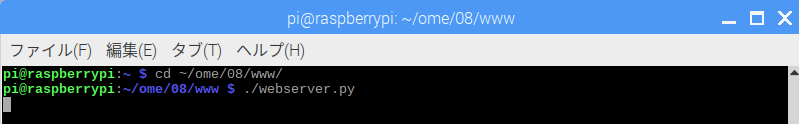
\includegraphics[width=13cm]{./text08-img/textbook-img063.png}

\end{center}
アクセスする際は、IPアドレスとともに3000番のポートを指定する必要があります。
起動したディレクトリがドキュメントルート(ウェブページやCGIプログラムから見たルートディレクトリ)になります。


実行した後はこのターミナルではウェブサーバが動いており、メッセージを表示するために使用をします。
\textbf{このターミナルは閉じないでください。}

ウェブページアクセス時のメッセージ例
:

もし、閉じてしまった場合はもう一度起動をしなおしてください。

\begin{center}
  % Unhandled or unsupported graphics:
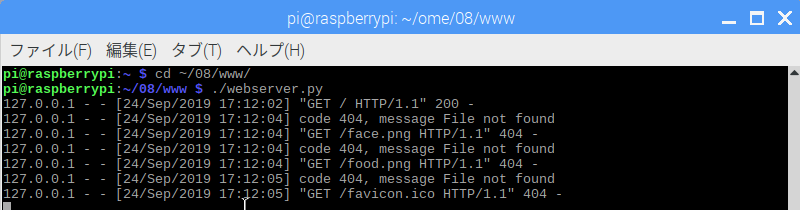
\includegraphics[width=13cm]{./text08-img/textbook-img064.png}

\end{center}
HSPのCGIプログラムはサーバー側(ウェブサーバが起動します)もしエラーが発生した場合には、ウェブサーバを起動したターミナルにエラーメッセージが表示されます。
ターミナルを確認してみてください。
エラーが発生したときはCGIプログラムは実行されません。

\begin{center}
  % Unhandled or unsupported graphics:
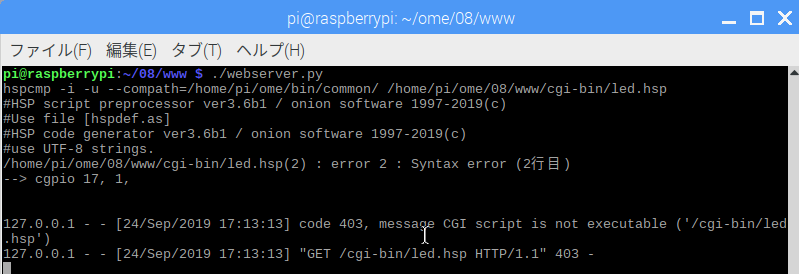
\includegraphics[width=13cm]{./text08-img/textbook-img065.png}

\end{center}
{\bfseries
ウェブサーバの停止方法}

\ruby{電源}{でんげん}を切る前、ウェブサーバが起動しているターミナルを閉じる前、ウェブサーバを停止したいときは、ウェブサーバを起動したターミナルを選択して

CtrlとCを同時に押します。



\begin{center}
  % Unhandled or unsupported graphics:
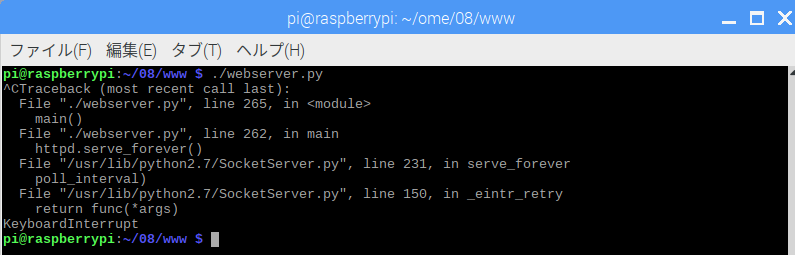
\includegraphics[width=13cm]{./text08-img/textbook-img066.png}

\end{center}
これでウェブサーバは終了します。

\section{\ruby{困}{こま}ったら質問フォームから質問しよう!}
質問フォームでは、授業でわからなかったことや確認したいことなどをホームページを通して質問できます。
たくさん質問してわからないことを解決しよう。

1.
ブラウザで\textbf{授業で使うホームページリスト}を開こう。

\textbf{授業で使うホームページリスト}は08フォルダの中のlinks.htmlです

リストの\textbf{子どもIT未来塾質問フォーム}をクリックして開いてくださいFigure~\ref{fig:refFigure0}。



% \begin{center}
% \begin{minipage}{10.88cm}


%   % Unhandled or unsupported graphics:
% 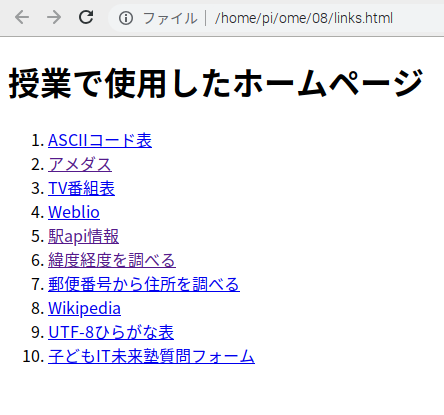
\includegraphics[width=6.638cm]{./text08-img/textbook-img017.png}



% Figure {\refstepcounter{Figure}\theFigure\label{seq:refFigure0}}:
% ホームページリストより質問フォームを開く
% \end{minipage}
% \end{center}




\begin{figure}[H]
  
    \begin{center}
      
      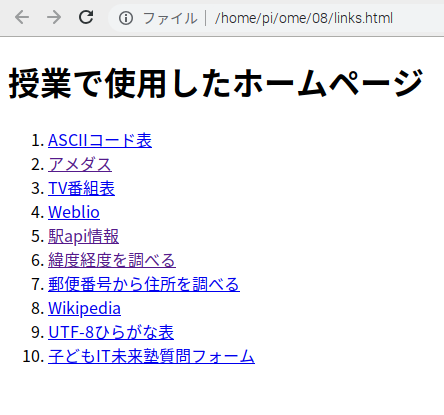
\includegraphics[width=6.638cm,height=6.204cm]{./text08-img/textbook-img017.png}
      \caption{\label{fig:refFigure0}ホームページリストより質問フォームを開く}
    \end{center}
    
\end{figure}

{\bfseries
スマートフォン等からの場合はhttps://bit.ly/2NHiVgiを開いてください。}


\bigskip

\clearpage

2.
クリックして開くと、質問フォームFigure~\ref{fig:refFigure1}が表示されます



% \begin{center}
% \begin{minipage}{0.9\textwidth}
% {\upshape
% 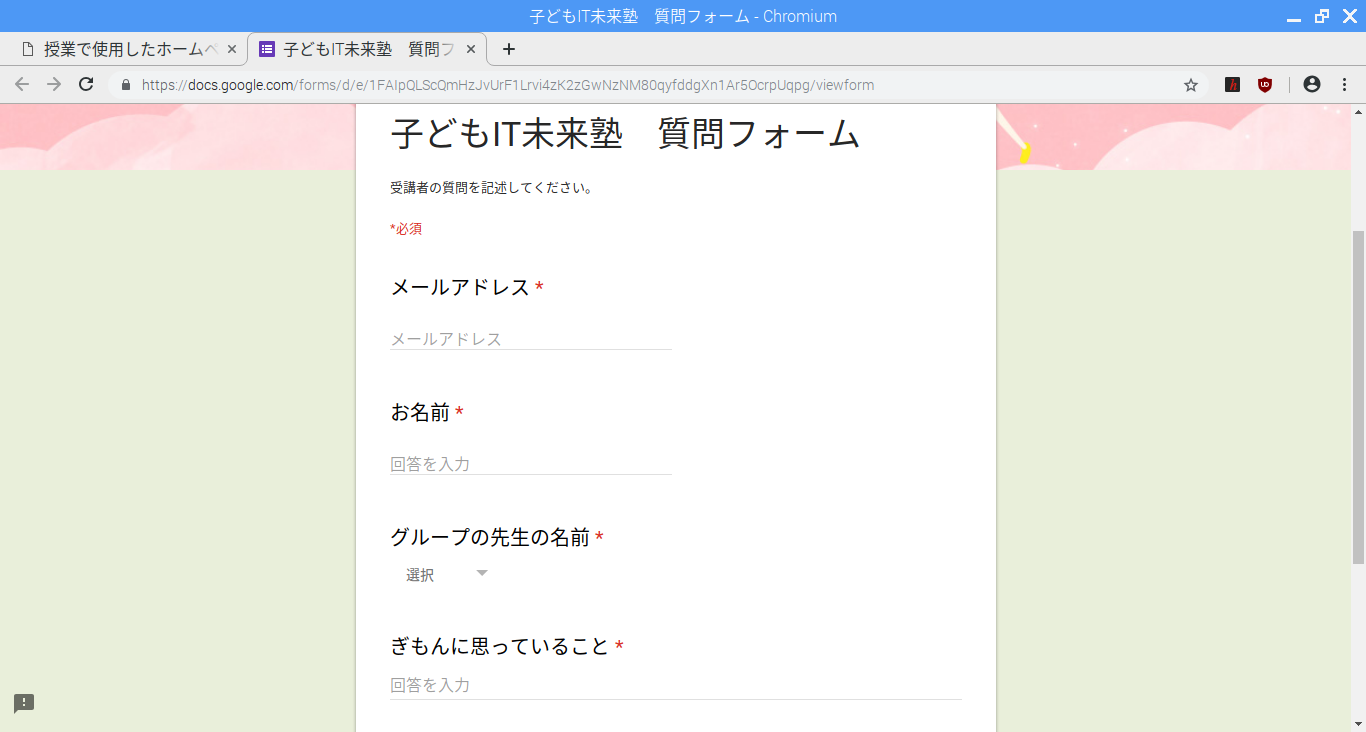
\includegraphics[width=\textwidth]{./text08-img/textbook-img067.png}
% \newline
% Figure {\refstepcounter{Figure}\theFigure\label{seq:refFigure1}}: 質問フォーム}
%   % Unhandled or unsupported graphics:
% \end{minipage}
% \end{center}


\begin{figure}[H]
  
    \begin{center}
      
      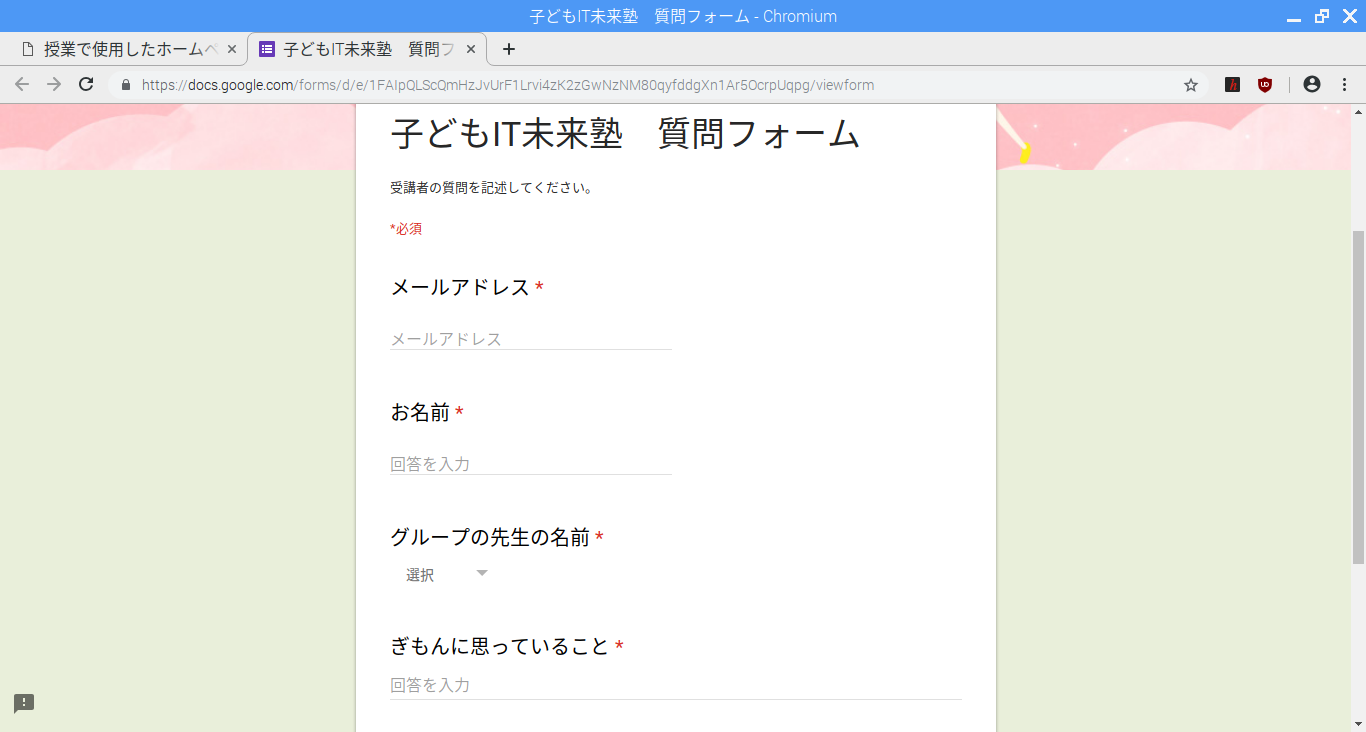
\includegraphics[width=\textwidth]{./text08-img/textbook-img067.png}
      \caption{\label{fig:refFigure1}質問フォーム}
    \end{center}
    
\end{figure}


\bigskip


メールアドレス、お名前、グループの先生の名前、ぎもんに思っていることを入力します。

気軽な質問でもOKです。

例 :



\begin{center}
  % Unhandled or unsupported graphics:
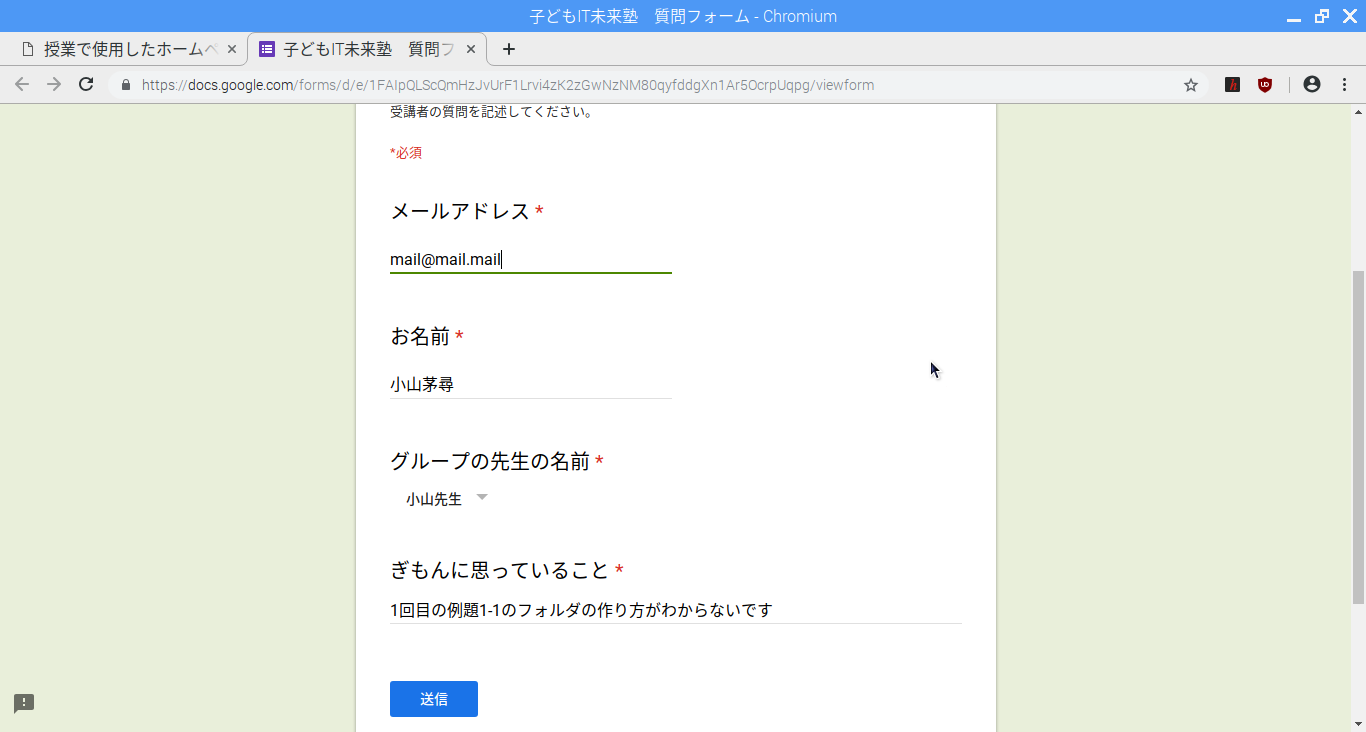
\includegraphics[width=0.9\textwidth]{./text08-img/textbook-img068.png}

\end{center}

\bigskip


\bigskip

\textbf{送信}を押すと質問が送られます。
Figure~\ref{fig:refFigure2}の画面が出たら質問は完了です。



% \begin{center}
% \begin{minipage}{0.9\textwidth}
% {\upshape
%    % Unhandled or unsupported graphics:
% 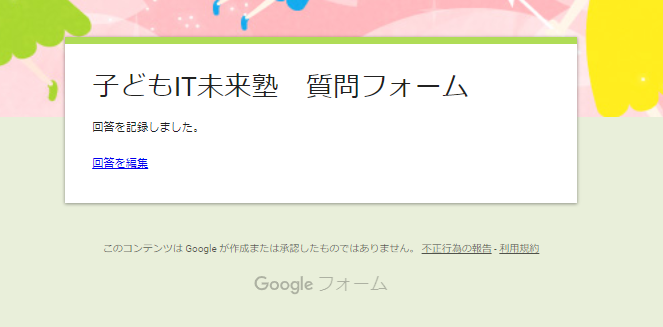
\includegraphics[width=\textwidth]{./text08-img/textbook-img069.png}
%  \newline
% Figure {\refstepcounter{Figure}\theFigure\label{seq:refFigure2}}: 質問送信画面}
% \end{minipage}
% \end{center}




\begin{figure}[H]
  
    \begin{center}
      
      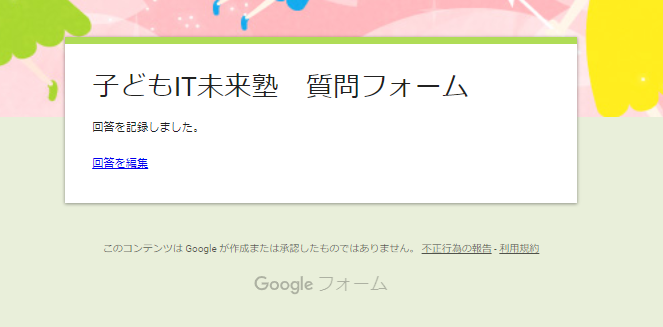
\includegraphics[width=\textwidth]{./text08-img/textbook-img069.png}
      \caption{\label{fig:refFigure2}質問送信画面}
    \end{center}
    
\end{figure}


メールアドレスのらんに入力したアドレスへグループの先生から回答メールがきます。

{\bfseries
\textmd{メールが来るまで、しばらくお待ちください。数日かかる場合があります。}}

\bigskip
\section{\ruby{参考文献}{さんこうぶんけん}}
HeartRails Express https://express.heartrails.com/api.html

